The iRPC chambers to be installed in stations RE3/1 and RE4/1 will demand changes, in comparison with the current chambers, in terms of design and electronics. The key design change is the finer gas gap thickness, from 2 mm to 1.4 mm~\cite{muon_tdr}, to reduce the intrinsic chamber threshold. In terms of electronics, a completely new FEB is being developed. This one should \textbf{(1) ensure the chamber efficiency in a high rate environment (up to 2 $kHz/cm^2$) and (2) provide information for a 2-dimensional readout}. 

\begin{wrapfigure}{r}{0.68\textwidth}
    \caption{\footnotesize Muon Efficiency versus High Voltage Effective (HVeff) and Total Current for the second version of FEB with PETIROC2B (FEBv1b) and the mean value of multiplicity for each side. "AND" efficiency showing without crosstalk impact. Scintillators placed in the HR of the chamber and covered about ~20cm. This setup includes three protected with leads scintillators inside GIF++ (w/o outside scintillators). Thresholds: $50\pm10$ $fC$.}\label{irpc_feb}

    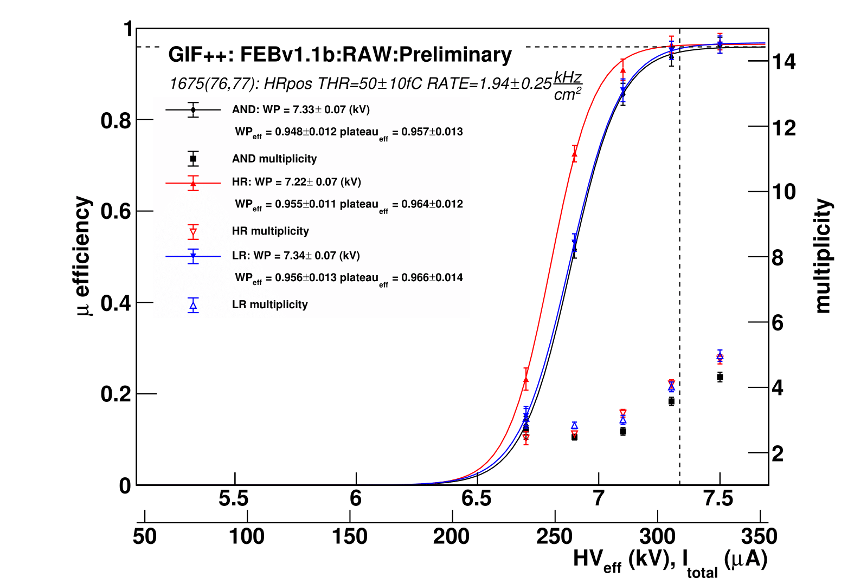
\includegraphics[width=0.68\textwidth, trim = {2.5cm 0 0.5cm 0 }, clip]{uioposter-images/irpc_feb_eff_v2}
\end{wrapfigure}

To achieve the requirements, the iRPC FEB will use PETIROC ASICs~\cite{petiroc}, with 32-channels each, for pre-amplification and discrimination of strip signals, providing low-jitter trigger with accurate charge and time measurements. Each strip end will be connected to one channel of the PETIROC. The digitized signal is sent to a FPGA (Field Programmable Gate Array), where a high resolution Time-to-Digital Converter (TDC) is implemented, allowing 2D measurement of the muon hit by measuring the arrival time difference of the two strip ends.

Currently there are two validated version of the iRPC FEB: FEBv0 (only one PETIROC2A and an Altera Cyclone II FPGA) and FEBv1 (with two PETRIOC2B and an Altera Cyclone V FPGA). Figure 3 shows the Muon Efficiency versus High Effective Voltage (HVeff, taking into account pressure and temperature effects) and the mean multiplicity, for cosmics data taken at GIF++ (CERN's Gamma Irradiation Facility - September-November 2019), considering the High Radius (HR), Low Radius (LR) strip ends and the logical AND of them. Future versions under development includes schematics closer to final version, radiation hard FPGA (PolarFire) and the possibility of a newer version of the PETIROC ASIC (2C, with automatic latching of individual channels).  

% % Plot V1 
% This plot shows s-curves with dependencies of Muon Efficiency versus High Voltage Effective (HVeff) for the second version of FEB with PETIROC2B (FEBv1b). Also, this slide showing the mean value of multiplicity for each side. AND efficiency showing without crosstalk impact. Data was taking during GIF++ (ATT=3.3) cosmic tests (September-November 2019). Scintillators placed in the HR of the chamber and covered about ~20cm. This setup includes three protected with leads scintillators inside GIF++ (without outside scintillators)
% HR: 500-480=20DACu. (50±10fC)

% LR: 500-480=20DACu (50±10fC)

% HIGH VOLTAGE EFFECTIVE (X-axis)

% Effective HV takes into account the change in pressure and temperature with respect to an HV reference value V0 at given pressure P0 and temperature T0.


% % Plot V2
% This plot shows s-curves with dependencies of Muon Efficiency versus High Voltage Effective (HVeff) and Total Current for the second version of FEB with PETIROC2B (FEBv1b). Also, this slide showing the mean value of multiplicity for each side. AND efficiency showing without crosstalk impact. Data was taking during GIF++ (ATT=46000) cosmic tests (September-November 2019). Scintillators placed in the HR of the chamber and covered about ~20cm. This setup includes three protected with leads scintillators inside GIF++ (without outside scintillators)
% HR: 500-480=20DACu. (50±10fC)

% LR: 500-480=20DACu (50±10fC)

% HIGH VOLTAGE EFFECTIVE (X-axis)

% Effective HV takes into account the change in pressure and temperature with respect to an HV reference value V0 at given pressure P0 and temperature T0.

% \begin{figure}
%     % Source: https://twiki.cern.ch/twiki/bin/view/CMSPublic/RPCUpgrade2020#iRPC_tests_Shchablo_Konstantin
%     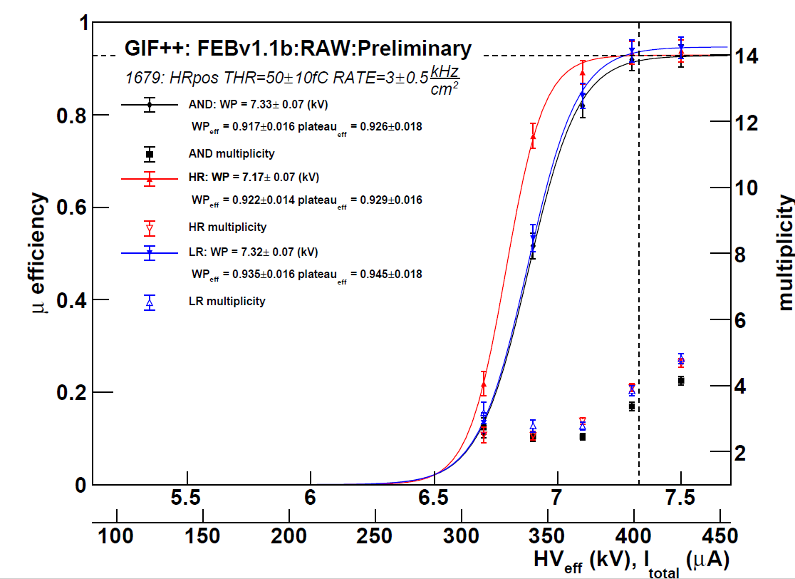
\includegraphics[width=1\textwidth]{uioposter-images/irpc_feb_eff}
%     \caption{\footnotesize A capition for iRPC FEB.}\label{irpc_feb}
% \end{figure}
